\section{Problem Analysis}

\begin{frame}{Manufacturer and Stakeholders}
\begin{itemize}
    \item \textit{Grundfos}
    \begin{itemize}
        \item Danish pump producer
        \item Sustainable solutions
    \end{itemize}

    \item Stakeholders
    \begin{itemize}
        \item List possible stakeholders
        \item Assign priorities
        \item Build influence/power-interest matrix
        \item Identify key stakeholders
    \end{itemize}
\end{itemize}

\end{frame}


\begin{frame}{Pumps and Impellers}
\begin{itemize}
    \item \textit{CR10} pump
\end{itemize}
% \begin{figure}
    \centering{
    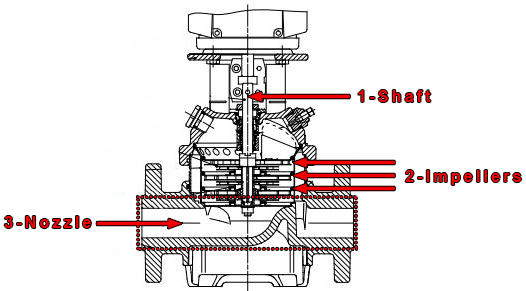
\includegraphics[width = 0.75\textwidth]{graphics/rebecca/CR10_pump}
    
    \tiny{(grundfos.com)}}
%     \caption{CR10 pump sectional drawing}
% \end{figure}

\end{frame}


\begin{frame}{Welding}
\begin{columns}

\begin{column}{0.6\textwidth}
\begin{itemize}
    \item Fibre laser
    \begin{itemize}
        \item Can be mounted on industrial manipulator
        \item Electrical efficiency
        \item Can weld stainless steel
    \end{itemize}
    \item Flat position
    \begin{itemize}
        \item Molten material within the boundaries
    \end{itemize}
\end{itemize}
\end{column}

\begin{column}{0.4\textwidth}
\begin{figure}
    \centering{
    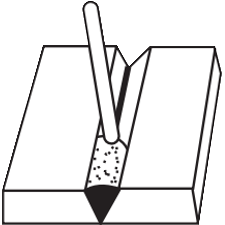
\includegraphics[width=0.9\textwidth]{graphics/rebecca/flat}
    
    \tiny{(M. I. Khan, Welding Science and Technology)}}
    % \caption{Flat welding position}
\end{figure}
\end{column}
\end{columns}
\end{frame}










\begin{frame}{Industrial Manipulators}{Andrej Orsula}
\centering
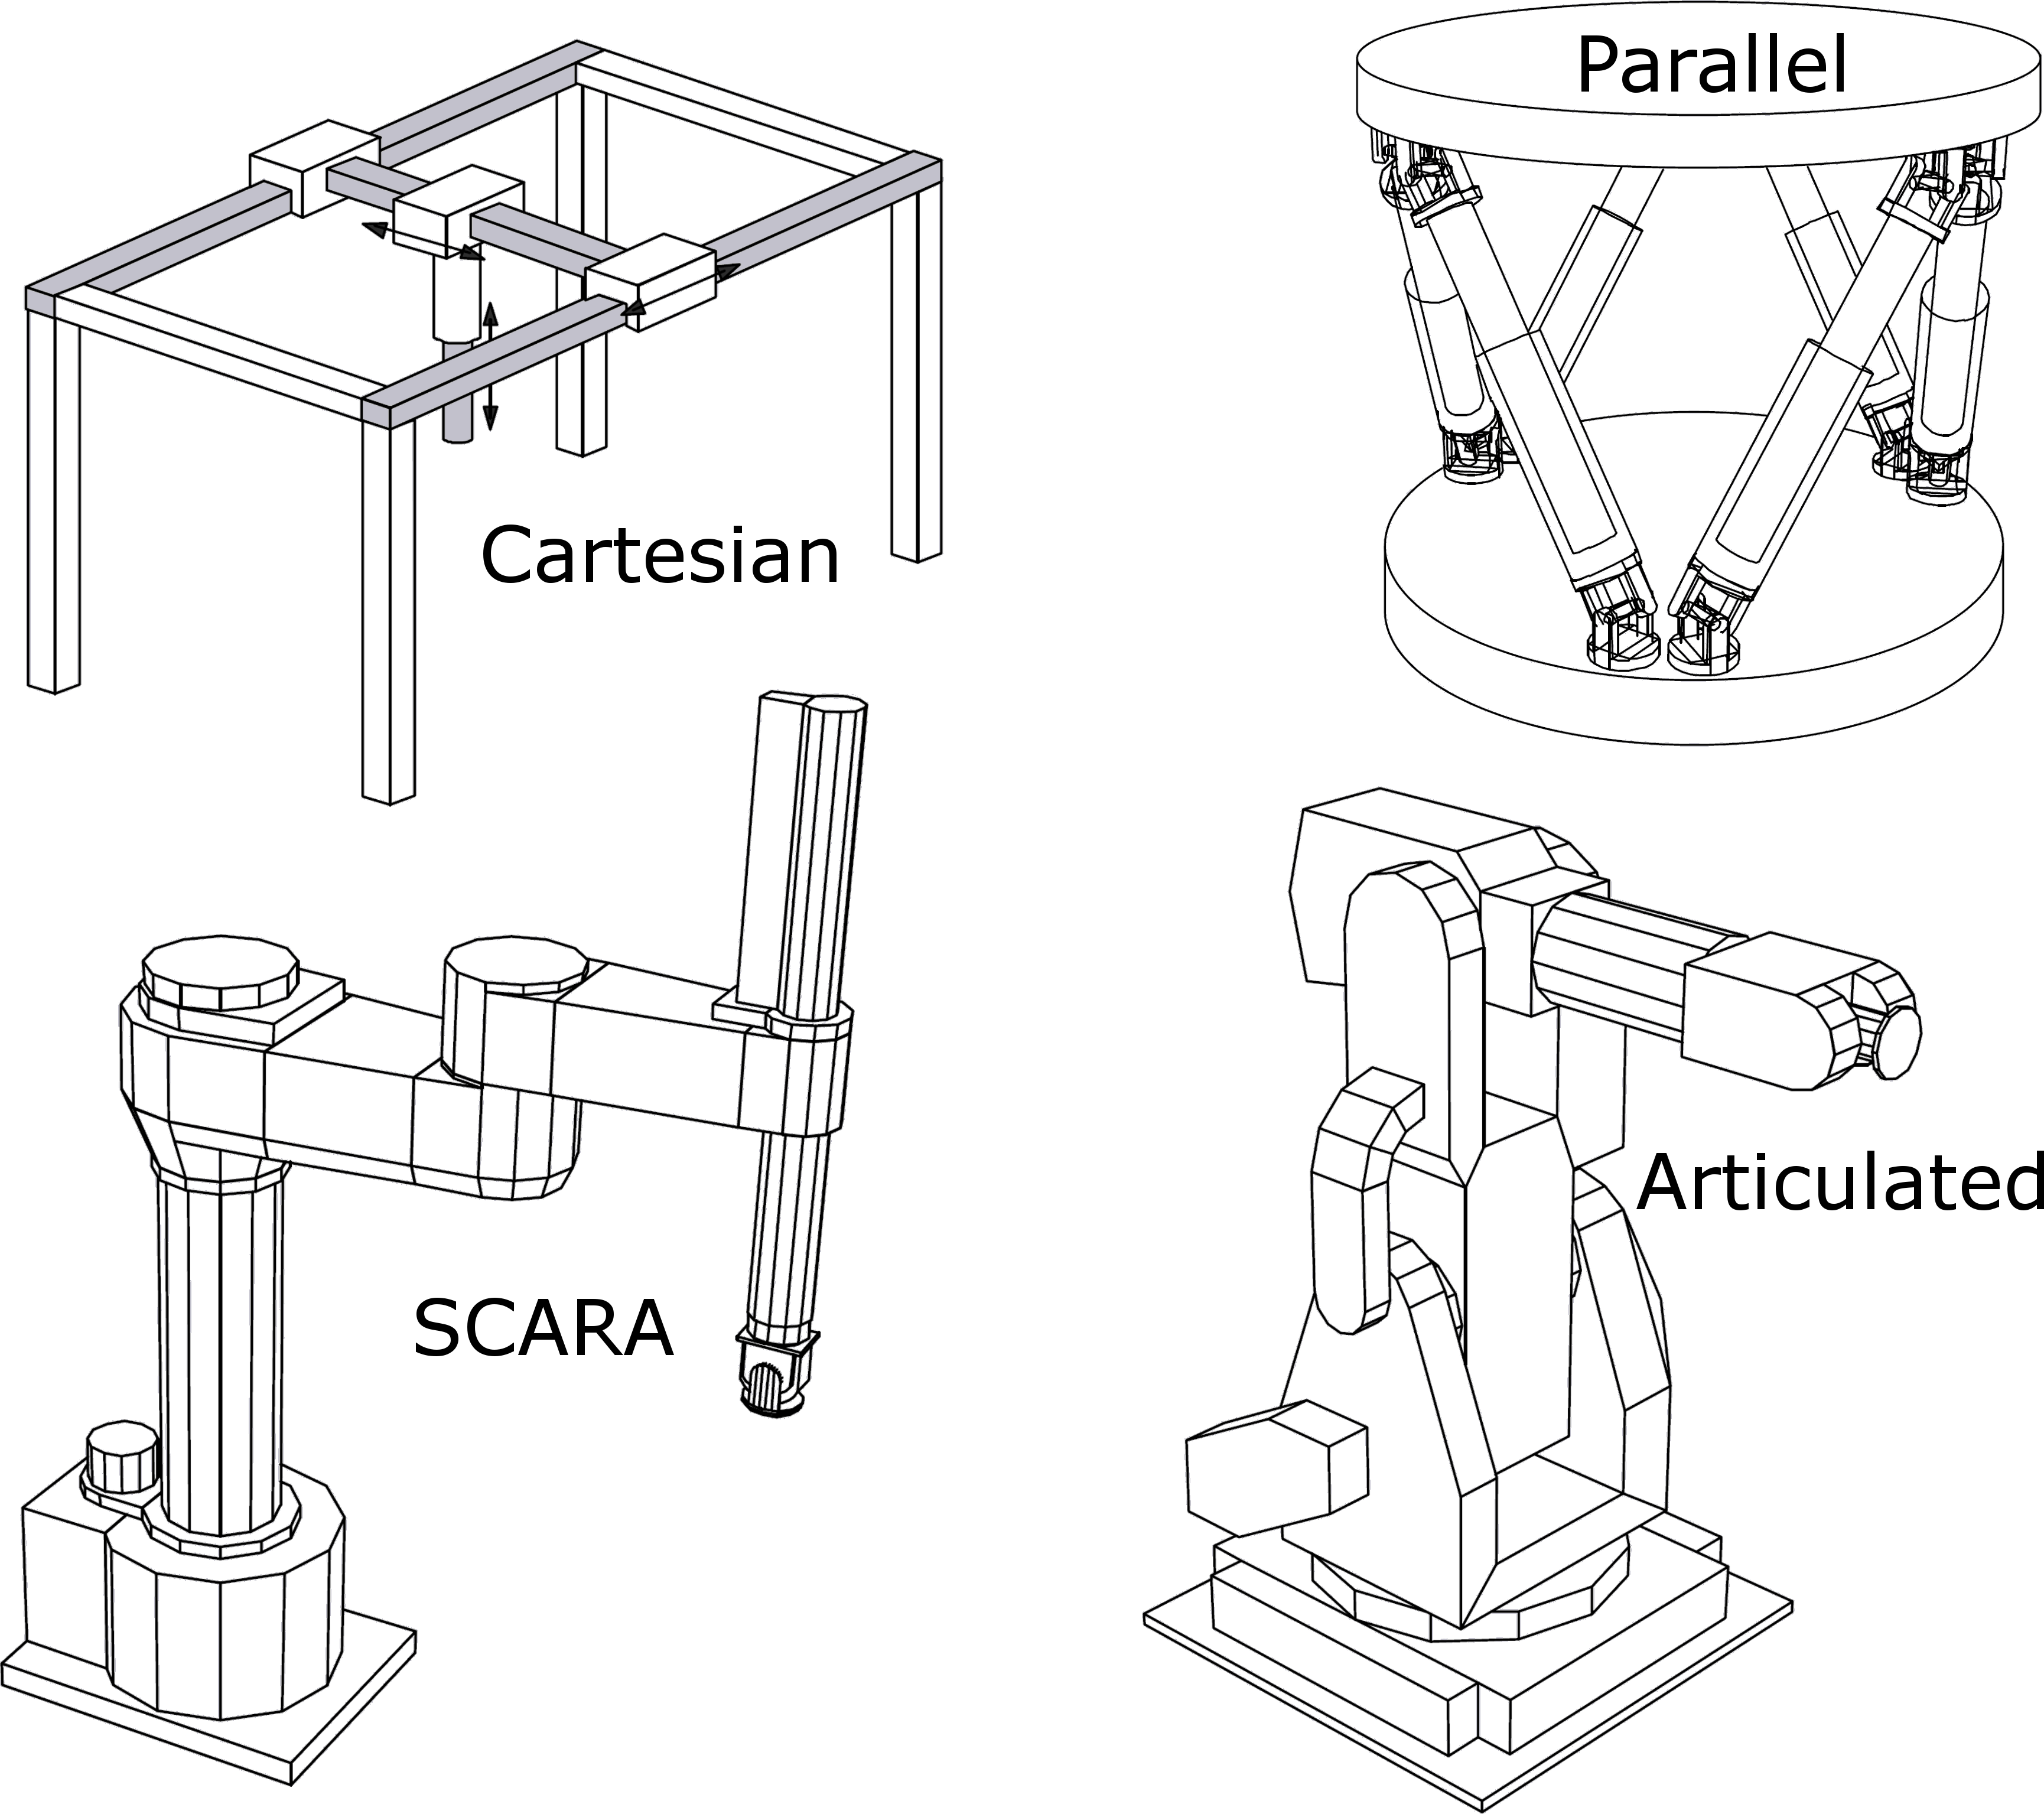
\includegraphics[width=0.785\textwidth]{graphics/andrej/indu_mani}

\tiny{(Springer Handbook of Robotics)}
\end{frame}



\begin{frame}{Safety}
\begin{columns}
\begin{column}{0.05\textwidth}
\end{column}
\begin{column}{0.40\textwidth}
Risk assessment
    \begin{itemize}
        \item Hazard identification
        \item Risk estimation
        \item Risk evaluation     
    \end{itemize}
\end{column}
\begin{column}{0.25\textwidth}
\begin{figure}[]
    \centering
    
\includegraphics[width=.9\textwidth]{graphics/andrej/arrow}
    \newline
\end{figure}
\end{column}
\begin{column}{0.3\textwidth}
Risk reduction
\end{column}
\end{columns}
\vspace{10mm}
\centering
\textit{International Organization for Standardization}
\end{frame}


% \begin{frame}{Safety}{\textit{International Organization for Standardization}}
%     \centering
%     \resizebox{\textwidth}{!}{
%     {\begin{tabular}{ll}
%       \hline \rowcolor{beamer@headercolor}\multicolumn{1}{c}{\color{white}{Standard}} & \multicolumn{1}{c}{\color{white}{Scope}} \\ \hline
% \textit{ISO 10218-1:2011} & Robots\\
% \rowcolor{beamer@barcolor} \textit{ISO 10218-2:2011} & Robot systems and integration\\
% \textit{ISO 11161:2007} & Integrated manufacturing systems\\
% \rowcolor{beamer@barcolor} \textit{ISO 11553-1:2005} & Laser processing machines\\
% \textit{ISO 12100:2010} & Risk assessment and risk reduction\\
% \rowcolor{beamer@barcolor} \textit{ISO 13849-1:2015} & Safety-related parts of control systems\\
% \textit{ISO 13850:2015} & Emergency stop function\\
% \rowcolor{beamer@barcolor} \textit{ISO 13854:1996} & Minimum gaps\\
% \textit{ISO 13857:2008} & Safety distances\\
% \rowcolor{beamer@barcolor} \textit{ISO 14119:2013} & Interlocking devices associated with guards\\
% \textit{ISO 14120:2015} & Guards\\
% \rowcolor{beamer@barcolor} \textit{ISO 60825-4:2007} & Laser guards\\
% \hline
%     \end{tabular}}}
% \end{frame}

% \subsection{Final Problem Statement}
\begin{frame}{Final Problem Statement}
% \begin{columns}
% \column{0.18\textwidth}
% \column{0.64\textwidth}
\begin{center}
How can a six-axis industrial manipulator and a fibre laser be used to weld the impeller from \textit{Grundfos}' \textit{CR10} pump?
\end{center}
% \column{0.18\textwidth}
% \end{columns}
\end{frame}